\documentclass[review]{acmsiggraph}
\usepackage{amssymb}
\usepackage{amsmath}
\usepackage{amsbsy}
\usepackage{wrapfig}
\usepackage{soul}
\usepackage{hhline}
\DeclareMathOperator*{\argmin}{arg\,min}

%% editing comment

%\newcommand{\cmt}[1]{\textcolor{red}{\textbf {#1}}}
\usepackage[usenames] {color}
\definecolor{purple}{rgb}{0.4,0.2,0.8}
\newcommand{\cmt}[1]{}
\newcommand{\note}[1]{\cmt{Note: #1}}
\newcommand{\karen}[1]{\textcolor{red}{{Karen: #1}}}
\newcommand{\original}[1]{\textcolor{blue}{{Original: #1}}}
\newcommand{\jie}[1]{\textcolor{blue}{{Jie: #1}}}
\newcommand{\alex}[1]{\textcolor{purple}{{Alex: #1}}}
\newcommand{\greg}[1]{\textcolor{green}{{Greg: #1}}}
\newcommand{\newtext}[1]{#1}
%\newcommand{\newtext}[1]{\textcolor{blue}{#1}}
\newcommand{\eqnref}[1]{Equation~(\ref{eqn:#1})}

%% ignore text
\long\def\ignorethis#1{}

%% abbreviations
\newcommand{\etal}{{\em{et~al.}\ }}
\newcommand{\eg}{e.g.\ }
\newcommand{\ie}{i.e.\ }

%% reference shortcuts
\newcommand{\figtodo}[1]{\framebox[0.8\columnwidth]{\rule{0pt}{1in}#1}}
\newcommand{\figref}[1]{Figure~\ref{fig:#1}}
%\renewcommand{\eqref}[1]{Equation~(\ref{eq:#1})}
\newcommand{\secref}[1]{Section~\ref{sec:#1}}

%% frequently used mathematical structures
\newcommand{\vc}[1]{\ensuremath{\mathbf{#1}}}
\newcommand{\pd}[2]{\ensuremath{\frac{\partial{#1}}{\partial{#2}}}}
\newcommand{\pdd}[3]{\ensuremath{\frac{\partial^2{#1}}{\partial{#2}\,\partial{#3}}}}


% math macros
\newcommand{\vEndEff}{\ensuremath{\vc{d}}}
\newcommand{\vRelMove}{\ensuremath{\vc{r}}}
\newcommand{\sSet}{\ensuremath{S}}


\newcommand{\vControl}{\ensuremath{\vc{u}}}
\newcommand{\vPoint}{\ensuremath{\vc{p}}}
\newcommand{\sSpringCoef}{{\ensuremath{k_{s}}}}
\newcommand{\sDamperCoef}{{\ensuremath{k_{d}}}}
\newcommand{\vHandle}{\ensuremath{\vc{h}}}
\newcommand{\vForce}{\ensuremath{\vc{f}}}

\newcommand{\mTransChain}{\ensuremath{\vc{W}}}
\newcommand{\mRotateTrans}{\ensuremath{\vc{R}}}
\newcommand{\sJoint}{\ensuremath{q}}
\newcommand{\vJoint}{\ensuremath{\vc{q}}}
\newcommand{\mJoint}{\ensuremath{\vc{Q}}}
\newcommand{\mMass}{\ensuremath{\vc{M}}}
\newcommand{\sMass}{\ensuremath{{m}}}
\newcommand{\vGravity}{\ensuremath{\vc{g}}}
\newcommand{\vConstr}{\ensuremath{\vc{C}}}
\newcommand{\sConstr}{\ensuremath{C}}
\newcommand{\vCOM}{\ensuremath{\vc{x}}}
\newcommand{\sGeneralForce}[1]{\ensuremath{Q_{#1}}}
\newcommand{\vStateVar}{\ensuremath{\vc{y}}}
\newcommand{\vControlVar}{\ensuremath{\vc{u}}}
\newcommand{\argmax}{\operatornamewithlimits{argmax}}
\newcommand{\tr}[1]{\ensuremath{\mathrm{tr}\left(#1\right)}}




%%%%%%%%%%%%%%%%%%%%%%%%%%%%%%%%%%%%%%%%%%%%%%%%%%%%%%%%%%%%%%%%%%%
%
% Here are a bunch of macros, mostly for math.
%
%%%%%%%%%%%%%%%%%%%%%%%%%%%%%%%%%%%%%%%%%%%%%%%%%%%%%%%%%%%%%%%%%%%

\renewcommand{\choose}[2]{\ensuremath{\left(\begin{array}{c} #1 \\ #2 \end{array} \right )}}

\newcommand{\gauss}[3]{\ensuremath{\mathcal{N}(#1 | #2 ; #3)}}

\newcommand{\pctab}{\hspace{0.2in}}
\newenvironment{pseudocode} {\begin{center} \begin{minipage}{\textwidth}
                             \normalsize \vspace{-2\baselineskip} \begin{tabbing}
                             \pctab \= \pctab \= \pctab \= \pctab \=
                             \pctab \= \pctab \= \pctab \= \pctab \= \\}
                            {\end{tabbing} \vspace{-2\baselineskip}
                             \end{minipage} \end{center}}
\newenvironment{items}      {\begin{list}{$\bullet$}
                              {\setlength{\partopsep}{\parskip}
                                \setlength{\parsep}{\parskip}
                                \setlength{\topsep}{0pt}
                                \setlength{\itemsep}{0pt}
                                \settowidth{\labelwidth}{$\bullet$}
                                \setlength{\labelsep}{1ex}
                                \setlength{\leftmargin}{\labelwidth}
                                \addtolength{\leftmargin}{\labelsep}
                                }
                              }
                            {\end{list}}
\newcommand{\newfun}[3]{\noindent\vspace{0pt}\fbox{\begin{minipage}{3.3truein}\vspace{#1}~ {#3}~\vspace{12pt}\end{minipage}}\vspace{#2}}



\newcommand{\key}{\textbf}
\newcommand{\fun}{\textsc}

%\def\shortcite{\def\citename##1{}\@internalcite}


% Local Variables:
% TeX-master: "paper"
% End:

\TOGonlineid{0000}



\TOGvolume{0}
\TOGnumber{0}
\TOGarticleDOI{1111111.2222222}
\TOGprojectURL{}
\TOGvideoURL{}
\TOGdataURL{}
\TOGcodeURL{}

\title{Simulating Animations of Human Dressing
}


\author{Alex Clegg \and Jie Tan \thanks{e-mail: jtan34@gatech.edu} %
\and Greg Turk \\ \\ Georgia Institute of Technology %
\and C. Karen Liu}

\pdfauthor{Alex Clegg, Jie Tan, Greg Turk, C. Karen Liu}

%% Keywords that describe your work.

\keywords{Bicycle simulation, balance control, reinforcement learning, neural networks.}


\begin{document}

%% The ``\maketitle'' command must be the first command after the
%% ``\begin{document}'' command. It prepares and prints the title block.

%%\teaser{
%%  \includegraphics[width=\textwidth]{images/HSwing}
%%  \caption{An H-shaped character does its morning exercises.}
%%  \label{fig:HSwing}
%%}
\maketitle

%% Abstract section.

\begin{abstract}
%Dressing is one of the most common activities in human society. Perfecting
the skill of dressing can take an average child three to four years of
daily practice. The challenge is primarily due to the combined difficulty
of coordinating different body parts and manipulating soft and deformable
objects (clothes). We present a technique to synthesize human dressing by
controlling a human character to put on an article of simulated clothing.
We identify a set of \emph{primitive actions} which account for the vast
majority of motions observed in human dressing. These primitive actions
can be assembled into a variety of motion sequences for dressing different
garments with different styles. Exploiting both feed-forward and feedback
control mechanisms, we develop a dressing controller to handle each of the
primitive actions. The controller plans a path to achieve the action goal
while making constant adjustments locally based on the current state of
the simulated cloth when necessary. We demonstrate that our framework is
versatile and able to animate dressing with different clothing types
including a jacket, a pair of shorts, a robe, and a vest. Our controller
is also robust to different cloth mesh resolutions which can cause the
cloth simulator to generate significantly different cloth motions. In
addition, we show that the same controller can be extended to assistive
dressing.

% Because the human dressing motion is difficult to animate or motion capture, the input motion does not need to be exact or complete (a few keyframes or pretend-dressing mocap). We develop a feedback controller that takes into account the state of cloth

\end{abstract}

\begin{CRcatlist}
  \CRcat{I.3.7}{Computer Graphics}{Three-Dimensional Graphics and Realism}{Animation};
  \CRcat{I.6.8}{Simulation and Modeling}{Types of Simulation}{Animation}.
\end{CRcatlist}

%% The ``\keywordlist'' command prints out the keywords.
\keywordlist
\copyrightspace


\section{Introduction}
\vspace{-0.1 in}
% \karen{Very high level comments: 1. Most problems mentioned in the
%   second paragraph are based on the assumption that animators use
%   physics simulation to generate cloth motion. We might want to
%   establish this assumption first by describing a general or
%   reasonable approach for creating cloth/human motion. 2. We want to
%   explicitly state the input of our system. 3. Our problem can be
%   viewed as path planning. It's very difficult because the cloth keeps
%   moving and the human body can easily self-collide. Further, we are
%   facing a very unique problem regarding human/cloth collision. Unlike
%   most navigation problems, our goal is not to avoid colliding with
%   cloth. Instead, our goal is to embrase and utilize contacts to
%   change the state of clothes in order to achieve the task. }

This paper describes a system for animating the activity of putting on
clothing.  Dressing is one of the most common activities that each of us
carries out each day.  Scenes of dressing are also common in live-action
movies and television.  Some of these scenes are iconic, such as the
``jacket on, jacket off'' drill in The Karate Kid (2010 version) or
Spiderman pulling his mask over his head for the first time.  Such
dressing scenes are noticeably absent in computer animated films.  Despite
the importance of dressing in our lives and in film, there is as yet no
systematic approach to animating a human that is putting on clothing.

% Mr. Rogers putting on his cardigan sweater in the children’s TV show,
% Mrs.  Robinson slipping on her stockings in The Graduate.
%
% The trailer for The Incredibles shows how far a computer animator will
% go to avoid showing a character pulling on their clothes.  

Our goal is to provide a system that will allow an animator to create
motion for a human character that is dressing.  We want the animator to
have a high degree of control over the look of the final animation.  To
this end, we desire a system that allows the user to describe the dressing scene as a sequence
of high-level actions.  Also, we would like our system to
accept approximated human motion, in either the form of keyframes or
motion capture, as reference for styles or aesthetics.  Thus the input from
the animator for a given dressing scene consists of: a character model,
a garment, a sequence of dressing actions, and reference
motions for the character. In order to create animation that is
physically plausible, we made the choice to use physical simulation of
cloth to guide the garment motions. By using cloth simulation, the
human figure, made of a collection of rigid segments, can interact
with the cloth in a natural manner.
 
% Our system takes these inputs from the animator and creates a physically
% realistic looking animation.  In order to create animation that is
% physically plausible, we made the choice to use physical simulation of
% cloth to guide the garment motions.  By using cloth simulation, the motion
% of the character affects the cloth motion in a natural manner.  We
% represent our human figures as a collection of rigid segments that are
% connected by joints.

% People use a wide variety
% of clothing types, including: shirts, pants, underwear, dresses, skirts,
% socks, shoes, hats, gloves, vests, jackets, and sweaters.

The essence of animating the act of dressing is modeling the
interaction between the human character and the cloth.  The human's motion
must adapt to the motion of the cloth, otherwise problems occur such as the
clothing slipping off or a hand getting stuck in a fold.  We often take
for granted the complex set of motions that are needed to put on our
clothes.  The seemingly simple act of putting on a jacket requires a
careful coordination between the person and the jacket.  Unconsciously we
make constant adjustments to our hand's position when inserting it into
the jacket's sleeve.  We hold our body at an angle to keep a sleeve from
sliding off our shoulder.  After putting on the first sleeve, we may use
any of several strategies to get our hand behind our back and within reach
of the second sleeve.  A system for animation of dressing must address
these kinds of complexities.

We have found that a small set of \emph{primitive actions} account for the vast
majority of the motions that a person goes through to put on an article of
clothing.  The approach that we take to dressing is to first have the
animator assemble a desired dressing motion from a small number of such
actions.  These actions include placing a hand or foot through an opening,
pulling the garment onto a limb, and stretching out a limb after it has
been positioned in the clothing.  Once this sequence of actions has been
assembled, producing the dressing animation can proceed.  The system steps
forward in time, updating the cloth's position through simulation.  The
character's motion during each of the actions are guided by optimization
and planning in order to satisfy the requirements of a given
action. The system adjusts the character's pose to match the end of one
action to the start of the next. Some portions of a dressing sequence do
not require the character to react to the cloth, and such segments can follow
the provided keyframe or motion capture data.

To a large degree, the problem that a dressing animation system must solve
is a form of \emph{path planning}. The character's body parts must move in coordination to
complete the task while preventing self-intersection and the
character must move in and around the cloth in such a way that the garment
ends up properly on the person. However, the dressing problem has a
few unique challenges which are not addressed by standard path planning
algorithms. Unlike typical path planning that avoids
collisions, contact between the body parts and the cloth is to be
expected. In fact, \emph{utilizing} contact to expand the opening of a folded
sleeve or fixate a part of cloth on the body is crucial for
successful dressing.

% To a large degree, the problem that a dressing animation system must solve
% is a form of \emph{path planning}.  First, the character's motion must not
% cause self-intersection between body parts.  We use several techniques
% for avoiding such collisions between body parts.  Moreover, the character
% must move in and around the cloth in such a way that the garment ends up
% properly on the person.  Some actions specifically require the character
% to react to the motion of the cloth.  Consider the case of trying to put a
% foot into the opening for one leg in a pair of pants.  Our system
% constantly adjusts the motion of the character's foot so that it draws
% closer to the opening without getting tangled in the cloth.  We accomplish
% this by using visibility information about the cloth to provide feedback
% that controls the limb's motion.  Note that this is not the typical form
% of path planning that would avoid colliding with the cloth.  Contact
% between the person and the cloth is to be expected.

Using our action-based dressing system, we have produced a variety of
animations of a character that is putting on various types of clothes.
This includes putting on a jacket, pulling on pants while sitting, putting
on pants while standing, dynamically swinging on a vest, and having one character assist another in putting on a robe.



\section{Related Work}

Interacting with surrounding humans or objects is an important research problem in character animation. Much previous research focused on close range interaction, which involves many challenging problems, such as collisions handling \cite{Ye:2012}, spatial constraints solving \cite{Ho:2010:SRP}, and path planning \cite{Kallman:2003,Yamane:2004:SAH,Bai:2012:SCO}. These existing techniques generated interesting animations beyond what simple forward simulation or keyframe interpolation can achieve. However, most methods assumed that the character interacts with humans or objects made of rigid bodies. Ho and Kumar \shortcite{Ho:2009:CMS} introduced a technique to interact with deformable bodies using topology coordinates, in which the topological relationship of the character's body and the environment can be easily controlled.

- Spatial Relationship Preserving Character Motion Adaptation
Path planning
- Synthesis of Concurrent Object Manipulation Tasks
- Planning collision-free reaching motions for interactive object manipulation and grasping
- Synthesizing animations of human manipulation tasks


Hand manipulation with soft objects
- Coupling Cloth and Rigid Bodies for Dexterous Manipulation
 Robotic cloth manipulation

Dexterous manipulation is a broad research area that has a vari- ety of applications in computer graphics and robotics. Although a precise definition is still open to interpretation, dexterous manipu- lation is typically defined as the use of multiple fingers to achieve a desired object configuration. In computer graphics, researchers have shown that intricate control strategies, such as finger gaiting [Ye and Liu 2012], rolling/sliding [Liu 2009; Bai and Liu 2014], or grasping/regrasping [Pollard and Zordan 2005; Kry and Pai 2006; Zhao et al. 2013; Wang et al. 2013], can be physically simulated on an anthropomorphic hand model. However, one of the most im- portant assumptions these techniques make is that the manipulated objects are rigid bodies with only six degrees of freedom.Manipulating deformable objects is a more challenging problem due to more degrees of freedom and more complex collision phenomena. Researchers in robotics have studied the problems of manipulat- ing fabric, cables, foam rubber, or sheet metal [Kosuge et al. 1995; Wu et al. 1995; Fahantidis et al. 1997; Osawa et al. 2007; Bersch et al. 2011; Miller et al. 2012]. Many previous approaches enhance control and planning algorithms by using simulation techniques to estimate the state of the deformable objects. For example, robotics researchers used a cloth simulator to approximate the contour of the clothes being folded by a PR2 robot [Cusumano-Towner et al. 2011]. Because the interaction between the robot hands and the cloth was relatively simple (i.e. grasping only), their simulation ap- plied position constraints to pin the cloth in the air instead of sim- ulating the hands. Our work aims to simulate the hands, the cloth, and their effects to each other realistically. We show that with a more accurate simulation routine, a wide variety of manipulation strategies can be achieved.


Cloth control without hands
- Manipulation of Flexible Objects by Geodesic Control
- Harmonic Parameterization by Electrostatics
Wojtan
Jernej


Papers that demonstrate dressing:
- Character Motion Synthesis by Topology Coordinates: They generated keyframes in topology coordinates and interpolate motion. The character does not respond to the state of the clothes. No autonomous control. They demonstrated that a character stretching the arms out of a piece clothes wrapped around it using keyframes. 
- Harmonic Parameterization by Electrostatics
- Clothing manipulation, Igarashi


Cloth sim interacting with rigids
- Coupling Cloth and Rigid Bodies for Dexterous Manipulation

\section{Overview}

\begin{figure}
  \centering
  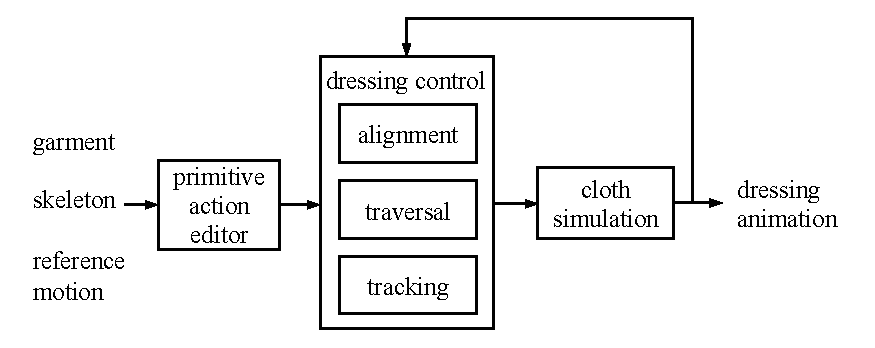
\includegraphics[width=3.3in]{images/overview}
  \caption{The overview of our system.}
  \label{fig:overview}
\end{figure}

\begin{table}
  \centering
  \begin{tabular}{|l|l|}
    \hline
    Action & Description \\
    \hline
    Grip(RH, $\vc{f}_{1}$) & Grip the colar feature $\vc{f}_1$  with the right hand.\\
    Track($\hat{\vc{q}}(t)$, $T_1$) & Track the reference motion $\hat{\vc{q}}$ for $T_1$ seconds.\\
    Align(LH, $\vc{f}_{2}$) & Align the left hand with the armhole $\vc{f}_2$.\\
    Drag(RH, $\{B_i\}$) & Drag the cloth along the left hand $B_1$, the left\\
    &                      arm $B_2$ and the left shoulder $B_3$.\\
    Release(RH) & Release the cloth from the right hand.\\
    Idle($T_2$) & Idle for $T_2$ seconds.\\
    Track($\hat{\vc{q}}$(t), $T_3$) & Track the reference motion $\hat{\vc{q}}$ for $T_3$ seconds.\\
    Align(RH, $\vc{f}_{3}$) & Align the right hand with the right armhole $\vc{f}_3$.\\
    Stretch(RH) & Stretching the right hand into the sleeve.\\
    Track($\hat{\vc{q}}$(t), $T_4$) & Track the reference motion $\hat{\vc{q}}$ for $T_4$ seconds. \\
    \hline
  \end{tabular}
  \caption{An example action queue for dressing the upper body of a character with a jacket.}
  \label{table:actionQueue}
\end{table}


We have designed a system that allows a virtual human character to put on various types of garments. Our system consists of three main components: action queue, dressing control the cloth simulation.
At each step, our system fetches an action from the queue,
executes its corresponding dressing controllers and simulates the physics of the cloth. Figure \ref{fig:overview} illustrates the main components of our system. 
Given a piece of garment, a character and a reference dressing motion, our system allows a user to decompose the entire
dressing sequence into a queue of high level actions. For example, putting an arm into a sleeve involves \emph{aligning} the hand with the armhole and
\emph{dragging} the cloth from the wrist to the shoulder. 
Table~\ref{table:actionQueue} shows complete action queue for putting on a jacket.
For each action, we design kinematic dressing controllers that determine desired end effector positions based on the current cloth states, solves IK problems for full body poses and plans a collision-free joint path to fulfill the action. 






\section{Garments}

% \karen{I still see inconsistent tense in one paragraph, ``we
%   selected'', ``we use'', etc.}
% \karen{Perhaps a careful pass just to catch tense inconsistency is needed.}
% \greg{I fixed the tenses in this paragraph, but have not done a global
% check.}

Our example garments are from the Berkeley Garment Library, and have been
edited to fit the size of our human character.  These example garments
are a jacket, a pair of shorts, a robe, and a vest.
The garments are modeled as a finite element mesh and their motion is
physically simulated
using the ARCSim cloth simulator \cite{Narain:2012:AAR}. We use linear
stretching and bending models and constitutive models derived from
measurements \cite{Wang:2011}. The collisions are detected using a
bounding volume hierarchy \cite{Tang:2010} and resolved with non-rigid
impact zones \cite{Harmon:2008}.

\paragraph{Garment Features.} For each garment we defined a set of cloth
features that are important for dressing control. A feature is a set of
vertices on the cloth mesh.  Each feature is either a target for a hand or
foot to align with, or a location for a hand to grasp.  For example, we
use the vertex loop of an armhole as a feature for the hand to target when
putting the arm into a sleeve.  Figure~\ref{fig:features} shows all the
features that we use for the jacket and the shorts.

\begin{figure}[!t]
  \centering
  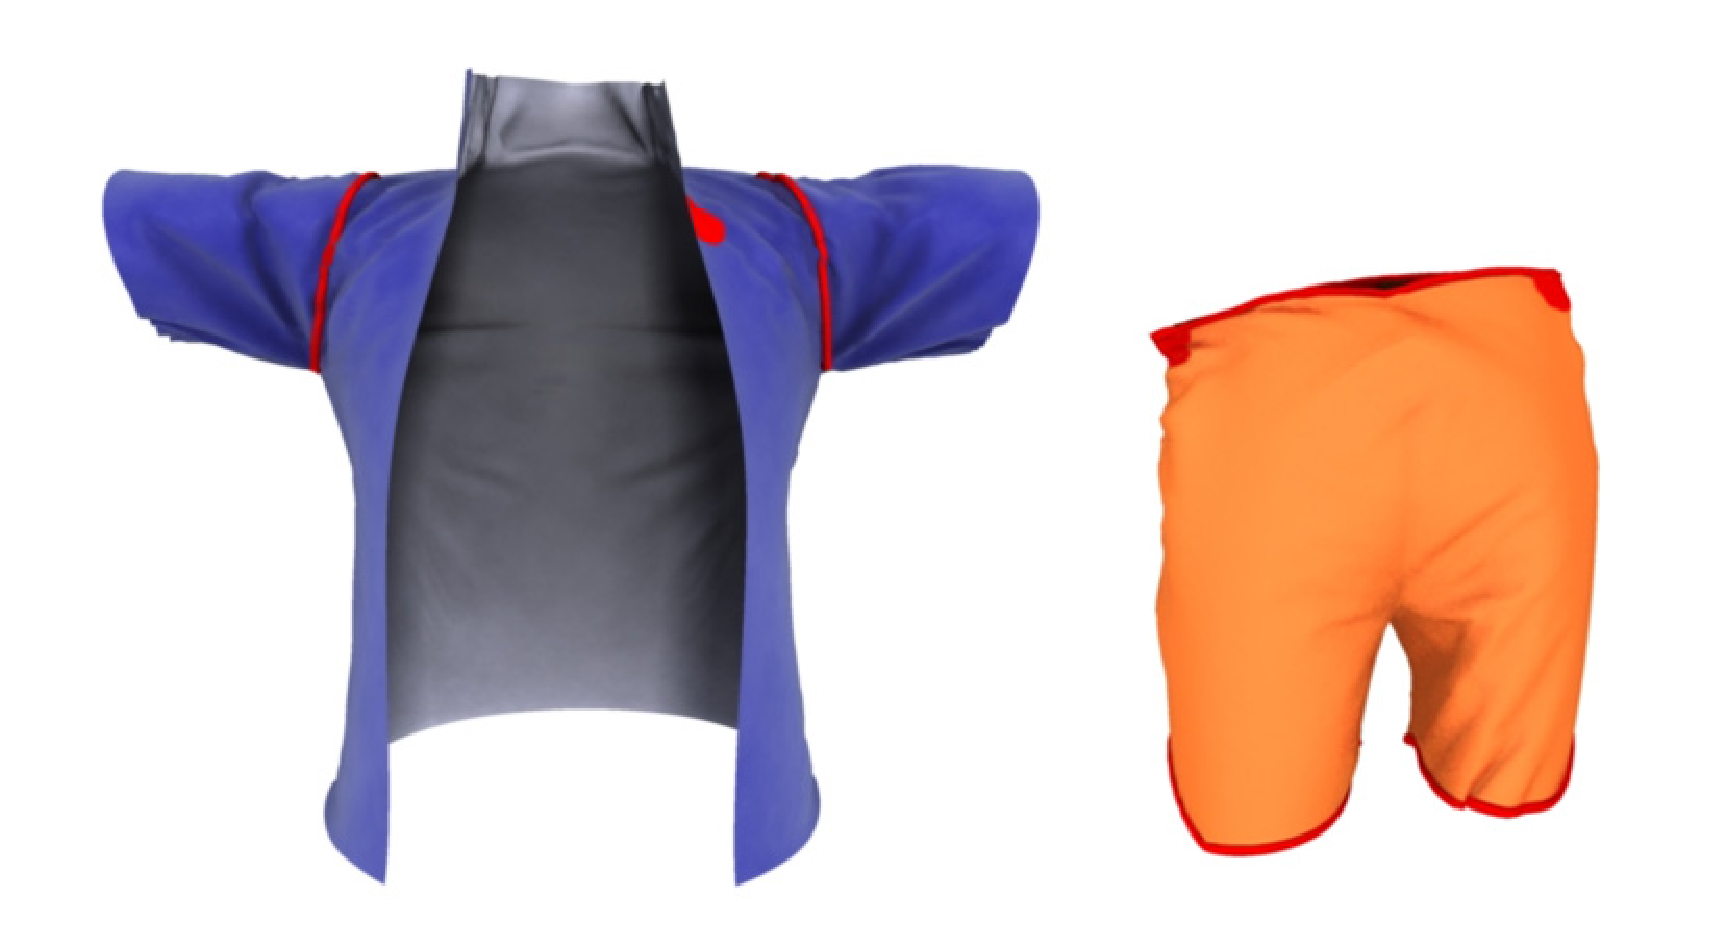
\includegraphics[width=3.5in]{images/features}
  \caption{Cloth features of a jacket and a pair of shorts that are used in dressing control. The red loops and patches are the features for alignment and grip respectively.}
  \label{fig:features}
\end{figure}


\section{Collision Free Inverse Kinematics}

We control the human character kinemactically in the dressing simulation. The kinematic control relies heavily on solving inverse kinematics (IK). A common formulation of IK is to solve the following optimization problem.

\begin{align}
\label{eq:IK}
  \min_{\vc{q}} & ||\vc{q} - \hat{\vc{q}}||_\vc{w}^2 \\
  \nonumber  \mathrm{subject\;} \mathrm{to} & \\
  \nonumber  &\vc{p}(\vc{q}) = \hat{\vc{p}}\\
\nonumber   &\vc{q}_{min} \leq \vc{q} \leq \vc{q}_{max}
\end{align}

where $\vc{q}$ are the joint angles, $\hat{\vc{q}}$ is the reference pose, $\vc{p}(\vc{q})$ are the end effector positions, $\hat{\vc{p}}$ are the target positions, $\vc{w}$ is a diagonal matrix that specifies the weight of each joint, $\vc{q}_{min}$ and $\vc{q}_{max}$ are the joint limits.

This optimization constrains the end effectors to be at the target locations and minimizes the pose deviation from the reference pose. However, this commonly used IK formulation does not prevent collisions between body parts. We find that with this formulation, collisions happen frequently during dressing because the end effectors need to navigate through a tight space between the body and the cloth. For this reason, we augment the optimization with an additional constraint to prevent interpenetrations between body parts. We approximate the collision volume of each body with multiple spheres and enforce no overlapping between pairs of spheres that belong to different body parts.

\begin{equation}
  ||\vc{c}_i(\vc{q}) - \vc{c}_j(\vc{q})||_2^2 - (r_1 + r_2)^2 \geq 0,\mbox{ if }B(i) \neq B(j)
  \label{eq:collision}
\end{equation}
where $\vc{c}$ and $r$ are the center and radius of the sphere, and $B(i)$ is the body part that the sphere belongs to.


\section{Dressing Control}

Our system allows a user to decompose the whole dressing sequence into multiple segments and specify high level actions for each segment (Table \ref{table:actionQueue}). We designed a small set of actions that are tailored for dressing control. The most important actions are alignment, traversal and tracking. 

\subsection{Alignment}
The first step to put on a cloth is to align one end effector with a cloth feature. For example, to align one hand with the armhole, or one foot with the belt loop. In alignment, we often choose a loop of vertices as the cloth feature and the goal is to control the end effector to pass through this loop. However, the target cloth feature is often folded and occluded by other parts of the cloth. It is not directly visable or reachable from the current end effector location. Furthermore, the alignment is a process of chasing a moving feature which has nonlinear dynamics and complex deformations. It is difficult to predict the movement of the feature and plan ahead. Even worse, as the end effector approaches the feature, it is highly likely that it will bump into the nearby cloth and knock the target away.  To address these challenges, we design a feedback controller for the alignment action.

\karen{Can we have an Algorithm (pseudo code) to summarize the following two paragraphs?}
Our alignment controller first finds an intermediate goal towards the target feature, and then move the end effector a small distance towards this goal in a way that minimizes the chance to knock away the target feature. These two steps are performed iteratively until the end effector successfully reaches the feature.

We set the intermediate goal as a vertex on the cloth which is visible from the end effector and it has the smallest geodesic distance to the target feature (Figure \ref{fig:geodesic}). However, the cloth geometry is represented as a single-layer triangular mesh, which means no difference between a point at the outer and the inner surface of the cloth. Since the end effector needs to reach the target feature from inside the cloth, we duplicate the mesh into two layers. These two layers are connected at their boundary. We precompute the geodesic distance on the two-layer cloth mesh using breadth first traversal starting from the feature vertices at the inner layer. At runtime, we find the unoccluded vertex with the minimal geodesic distance using rasterization techniques. We place a camera at the end effector and render the geodesic distance on the cloth mesh into a cubic environmental map. The brightest pixel on the map corresponds the direction to the intermediate goal. Note that we choose to render all six directions of the cubic map, which not only allows the end effector to move forward, but also sideways and backtrack. We find that the ability to detect the intermediate goal behind the end effector drastically increases the success rate of the alignment.

Given the intermediat goal $\vc{p}_g$ and the current end effector location $\vc{p}^n$, we set the desired end effector location $\hat{\vc{p}}$ at the next time step to be 
\begin{equation}
  \hat{\vc{p}} = \vc{p}^n+\alpha(\vc{p}_g - \vc{p}^n)
  \label{eq:target}
\end{equation}
where $\alpha$ is the step size that is specified by the user.

We found that in addition to the end effector location, its orientation also plays an important role in the alignment action. Since the end effector needs to navigate through a tight and winding space between folds of the cloth, its orientation should be aligned with the moving direction. This way of moving reduces the space swept by the end effector, lowers its chance to collide with nearby cloth and minimizes the normal impacts if collisions happen. For this reason, we add the following objective to the optimization (Equation~\ref{eq:IK}). \karen{What is the reference pose in Equation 1 used during alignment?}

\begin{displaymath}
E_{orientation} = 1-\frac{(\vc{p}_g-\vc{p}^n)^T}{||\vc{p}_g-\vc{p}^n||_2}\vc{d(q})
\end{displaymath}
where $\vc{d(q)}$ is the direction from the center to the tip of the end effector.

In addition, we also limit the joint speed within a certain threshold to ensure the smoothness of the motion.
\begin{displaymath}
-\dot{\vc{q}}_{thresh} \leq \frac{\vc{q} - \vc{q}^n}{\Delta t} \leq \dot{\vc{q}}_{thresh}
\end{displaymath}
where $\vc{q}^n$ is the current pose, $\Delta t$ is the time step, and $\dot{\vc{q}}_{thresh}$ is the maximum allowed speed.

To determine whether the alignment action has succeeded, we first find a plane that best fits the cloth feature.We then project the center of the end effector and the vertex loop of the feature onto this plane. If the center of the end effector has passed over this plane and the projected center is within the projected feature loop, the alignment has succeeded and we move on to the next action in the queue.

\subsection{Traversal}
After alignment, the center of the end effector has passed the desired cloth feature. However, at this point, the feature can still easily fall out of control due to gravity or inappropriate end effector motions. We design a traversal action to secure the alignment, which enables the end effector to pass throught the opening entirely and further into the cloth tubes. Examples of traversal include stretching an arm into a sleeve and dragging the pants up to the waist. To accomplish this action, we first compute a series of desired poses of the end effector or the whole limb. We then solve the collision-free IK for their corresponding full body poses, which are used as keyframes of the entire traversal motion. Although these keyframes are free of self collision among body parts, directly interpolating them can lead to inter-body penetrations. For this reason, we apply bi-directional Rapidly Expanding Random Tree (RRT) \cite{} to find a collision free trajectory between adjacent keyframes.

We observed that in daily dressing activities, the traversal action can be categorized into two types. In the first type, the limb to be dressed remains relatively motionless while another limb \emph{drags} the cloth along it. For example, the character uses its hands to drag the pants up along the legs. In the second type, the limb \emph{stretches} itself to pass through the tubular part of the cloth without assistance from other limbs. This situation is often seen when putting on the second sleeve of a jacket. To accomodate both types of travesal, we designed different desired poses of the end effector or the limb.

\paragraph{Dragging.} In the first case, a user can specify one end effector to drag the cloth and a set of body parts $\{B_1 ,..., B_n\}$ that the cloth should be dragged upon. We use the positions of the parent joints of those bodies as path nodes. For example, if the character is using his right hand to dress the left arm, the path nodes are the left wrist, the left elbow and the left shoulder (Figure \ref{}). For each of the path node $\vc{p}_i$, we set the target end effector location $\hat{\vc{p}}=\vc{p}_i$ in Equation~\ref{eq:IK}, and solve the collision-free IK for one keyframe of the dragging motion. 

\paragraph{Stretching.} In the second case of traversal, one limb straightens into the cloth tube without assistance from other end effectors. While the limb is stretching, another body part needs to keep the cloth from moving with the limb. We call this body part a \emph{fixture node}. For example, when stretching an arm into a sleeve as shown in Figure \ref{}, the fixture node is the opposite shoulder. We implemented the fixture node as an additional constraint in the optimization (Equation~\ref{eq:IK}).

\begin{align}
  \label{eq:fixtureNode}
  \vc{R}(\vc{q})& = \vc{R}^n\\
  \nonumber  \vc{t}(\vc{q})& = \vc{t}^n
\end{align}
where $\vc{R}^n$ and $\vc{t}^n$ are the current rotation and translation of the fixture node.

Besides the fixture node, a correct stretching direction is also critical to a successful stretching action. We used the direction from the center of the fixture node to the current end effector location as the stretching direction. Along this direction, the friction force caused by the stretching limb is canceled by the cloth tension pulled from the fixture node. This prevents the cloth feature from moving with the end effector so that the limb can further pass through the feature. We add an objective term to Equation \ref{eq:IK} to specify the desired stretching direction.
\begin{equation}
  E_{stretch} = 1 - \hat{\vc{d}}^T\vc{d(q)}
  \label{eq:stretching}
\end{equation}
where $\hat{\vc{d}}$ is the desired stretching direction and $\vc{d(q)}$ is the direction from the root to the tip of the limb.

We solve the collision-free IK with the additional objective (Equation~\ref{eq:stretching}) and constraint (Equation~\ref{eq:fixtureNode}), which gives us a key frame of full body pose for the stretching motion.


\subsection{Tracking}

To preserve the dressing style specified by the user, We use the tracking action to follow the reference motion $\hat{\vc{q}}(t)$. In most cases, it simply uses the next pose in the reference.
\begin{displaymath}
\vc{q} = \hat{\vc{q}}^{n+1}
\end{displaymath}
However, after alignment and traversal, the joint trajectory of the character could deviate far from the reference motion. Interpolation from the current pose to a pose in the reference is necessary for a smooth animation. To prevent inter-body collisions during the interpolation, similar to the dragging controller, we apply RRT \cite{} to find a collision free path and then follow this path to the target pose.

\subsection{Other Actions}

\paragraph{Grip and release.}
The grip action models the grasping of the character's hand. The cloth feature moves together with the character's hand if it is gripped. This action constrains the vertices in the cloth feature to the local frame of the end effector.
\begin{displaymath}
\vc{p}_w = \vc{Rp} + \vc{t}
\end{displaymath}
where $\vc{p}_w$ is the world coordinate of a vertex in the cloth feature, $\vc{p}$ is the local coordinate of this vertex at the end effector's frame, $\vc{R}$ and $\vc{t}$ are the rotation and translation of the end effector. The release action simply removes the above constraints and the cloth feature no longer moves with the end effector once it is released.

\paragraph{Idling.} This action freezes the character's motion for a user-specified time period. The main purpose of this action is to wait the clothes to settle before proceeding to the next dressing action.


\section{Results}
\begin{table}[b]
  \centering
  \begin{tabular}{|l|c|c|c|c|c|}
    \hline
    examples 		& cloth 	& act- 	& anim	& sim 		& control \\
                    & triangles & 	ions& time 	& time 		& time \\
    \hline
    jacket 			& 23.2k  	& 10	& 18s 	& 30h23m	&  14m  \\
    jacket (low res)& 2.7k		& 10	& 18s	& 2h58m		& 1m \\
    shorts (sitting) 	& 14.9k 	& 10	& 16s 	&  8h41m 	& 4m \\
    shorts (standing)	& 14.9k 	& 10	& 15s	&  7h52m	& 3m \\
    vest 			& 6.57k		& 14	& 13s	&  3h53m	& 1m   \\
    robe 			& 31.7k 	& 11	& 14s	& 20h40m	& 19m  \\
    \hline
  \end{tabular}
  \caption{Parameters and performance of the examples. cloth triangles: the number of elements in cloth simulation. Actions: number of actions. Anim time: wall clock time (in seconds) of the dressing animation. Sim and control times are the total times for the cloth simulation and our control functions respectively.}
  \label{table:data}
\end{table}


In this section we describe the results of our system. We chose four different types of garments from the Berkeley Garment Library, edited them to meet our needs, and put them on the character using different styles. Please watch the accompanying video for the dressing animations. Our system was implemented in C++. We used DART \cite{Liu:2012:STM} for human character modeling and ARCSim \cite{Narain:2012:AAR} for cloth simulation. We used a denim material profile with 3-4x thickening to simulate layered clothing articles. The examples were run on a desktop workstation with a 4-core 3.7 GHz CPU and 8 GB of memory. The typical running time of a dressing example is several hours to a day. The cloth simulation is the most time-consuming part and takes significantly longer than control. The parameters and performance data of our examples are summarized in Table
 \ref{table:data}. 


\paragraph{Jacket.} Figure~\ref{fig:jacket} shows a character putting on a
jacket using a common style: Put the left arm in its sleeve, swing the right arm to the back, find the hanging sleeve, and stretch the arm into it. The reference human motion for this style is made up of six keyframes. As shown in the video, dressing by directly playing back the reference motion without any feedback control fails to put on even the first sleeve. After gripping the collar of the cloth, our system first tracks the reference motion to a particular keyframe and then performs an alignment action. The character aligns his left hand with the corresponding armhole. Once the alignment is successful, the traversal action is executed. The character uses his right hand to drag the cloth up the length of the left arm. At the end of traversal, the right hand reaches the shoulder and releases the cloth. The character then swings his right arm to the back by tracking the reference motion. The second alignment phase begins when the character's right hand starts to search for the opening of the sleeve. This alignment phase is more challenging because the target armhole is completely occluded by multiple layers of cloth. The alignment action gradually finds better intermediate goals that are closer to the target feature and guides the hand to wiggle through the cloth folds towards the goal. 

In the jacket example we observed interesting emergent behavior, such as a natural exploratory gesture that is often used by humans to sort out the tangled cloth in dressing. Furthermore, the hand operates within a tight space between the pelvis and the hanging cloth during alignment. Without the collision-free IK, the hand or arm would penetrate the torso before aligning with the armhole. After the alignment, the character uses the traversal action to stretch the right arm into the sleeve and then tracks the reference motion until the jacket is completely on the body. 

A common challenge in cloth simulation is that the simulation may produce
drastically different motions if the resolution of the cloth changes. To
test the robustness of our system, we used the same actions to put on a
low resolution jacket with approximately 10x fewer triangles. Our system
was able to automatically adapt to the change in resolution and the
resulting differences in cloth motion without any manual tuning. Note that
the more coarse resolution cloth has fewer wrinkles and folds.  A
consequence of this is that the lower resolution jacket has a less occluded
armhole, so the right hand alignment phase is shorter in this sequence.

\paragraph{Vest.} We simulated putting on a vest in a more dynamic style (Figure~\ref{fig:vest}). We chose this example to demonstrate that using a small set of primitive actions, our system is able to put on a garment in a different style by using a different reference motion. Tracking the motion captured reference, the character swings the vest around his neck, then aligns the left hand with the corresponding armhole while the vest is swinging in mid-air. This alignment shows that our feedback control is robust and able to align not only with a target feature that is occluded by layers of cloth, but also with one that is moving quickly. Once the first arm is dressed, the right hand is aligned with the second armhole and stretches into it. 

\begin{figure*}[!t]
  \centering
  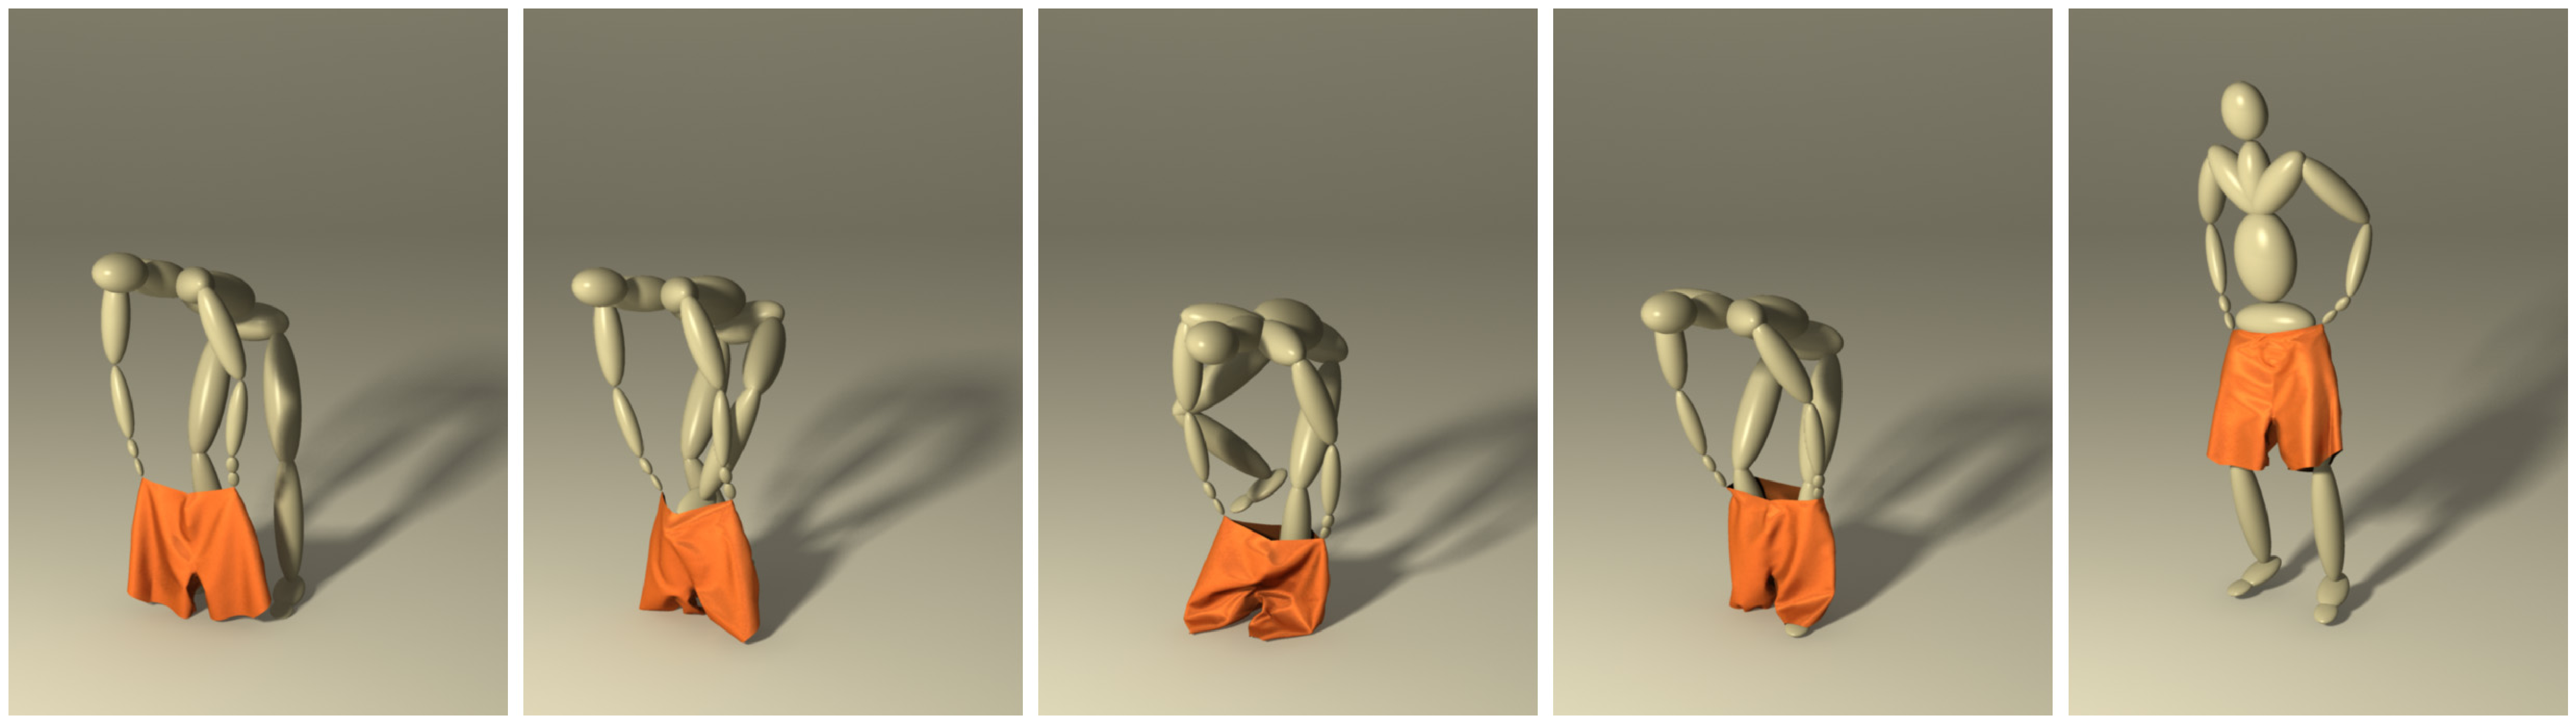
\includegraphics[width=\textwidth]{images/shortsStanding}
  \caption{A character puts on a pair of shorts in a standing pose.}
  \label{fig:shorts2}
\end{figure*}

\begin{figure*}[!t]
  \centering
  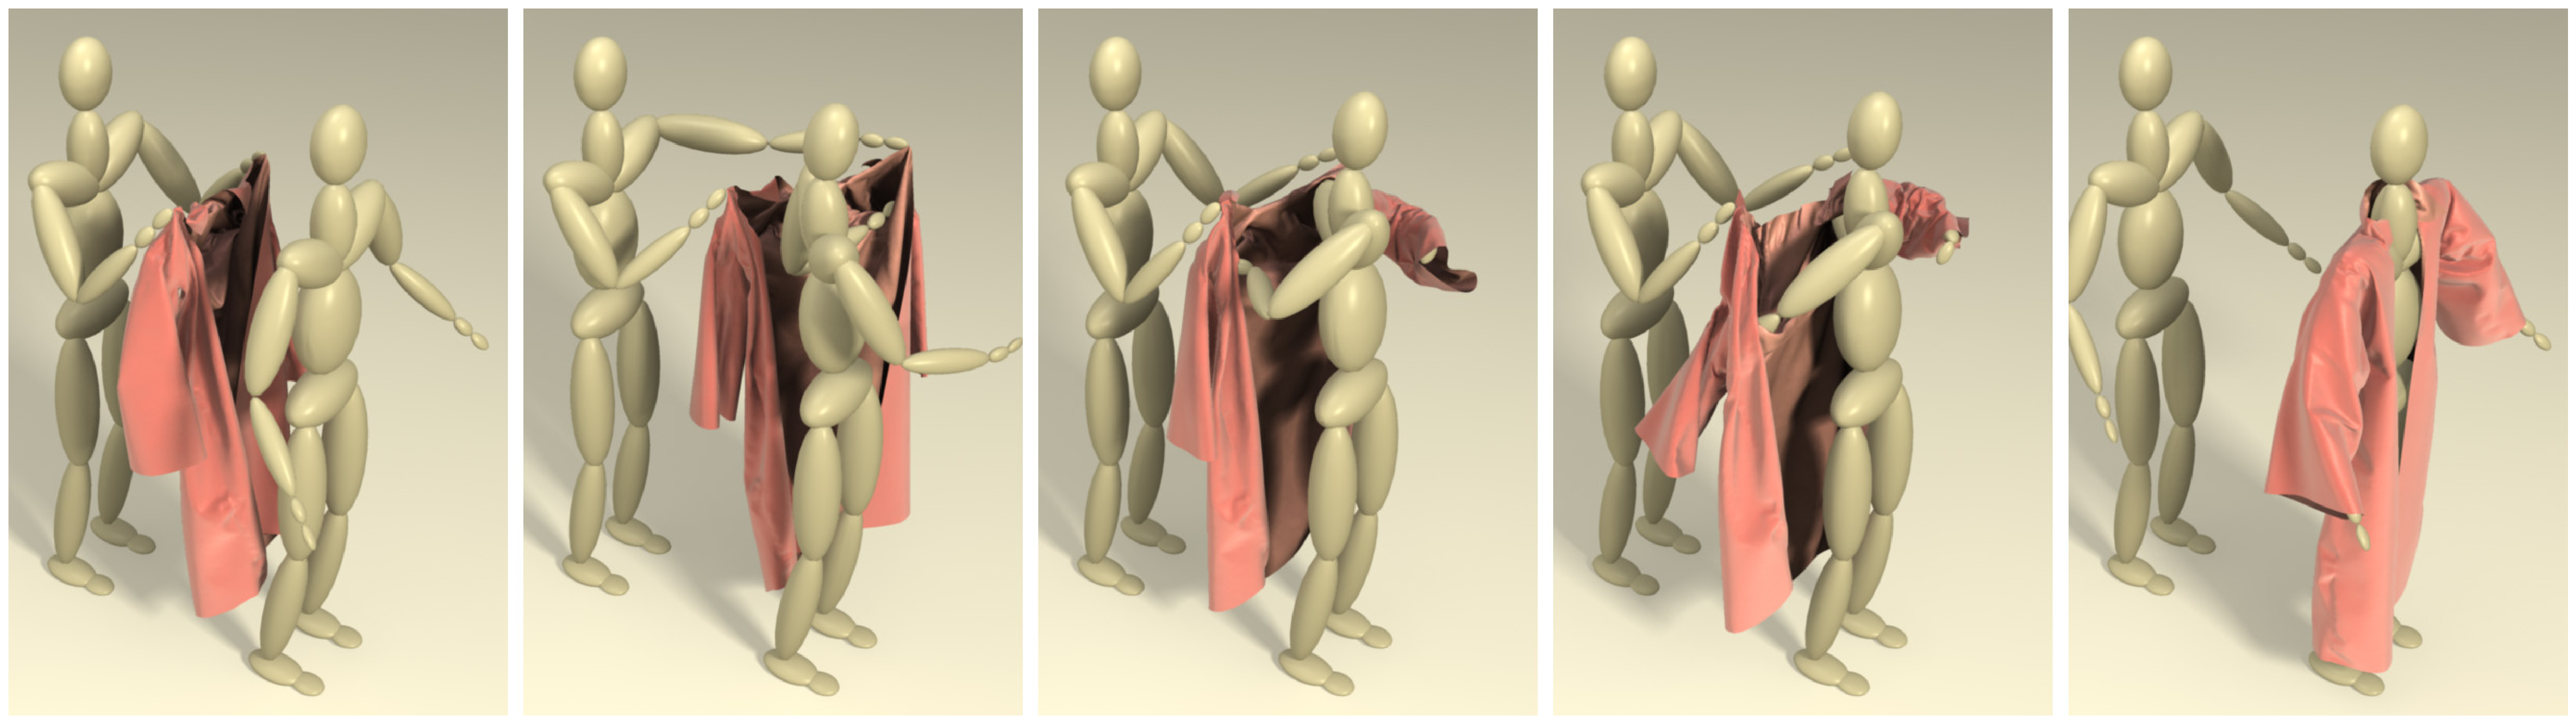
\includegraphics[width=\textwidth]{images/robe}
  \caption{A character puts on a robe with the help from another character.}
  \label{fig:robe}
\end{figure*}

\paragraph{Shorts.} Figure~\ref{fig:shorts1} demonstrates a character that
is putting on a pair of shorts in a sitting position. We used a motion
capture sequence as the reference motion in this example. The character
grips the waistband and leans forward by tracking the reference motion. He
first aligns his left foot with the waistband and then aligns it with the
bottom of the shorts' left leg. Similar alignment actions are applied to
the right foot. Once both feet are aligned with the desired features, the
character follows the reference motion to stand up and pull up the shorts.
The accompanying video shows that without the feedback control, the
character fails to put the feet into the shorts and ends up not wearing
the pants.

We also tested the generality of our system by using a different reference motion, in which we mocaped a person that is putting on a pair of shorts in a standing position. Despite the different style, we were able to reuse the action queue from the sitting shorts and successfully dress the lower body of the character (Figure \ref{fig:shorts2}).

\paragraph{Robe.} To show that our system can be used outside of the realm of self-dressing, we applied our method to an assisted dressing scene in which one character aids another in putting on a robe (Figure \ref{fig:robe}). The reference motion for this scene consists of five keyframes. First, the dressing character tracks the reference motion, twisting to the left and aligning his left hand with the armhole. After he straightens his arm into the sleeve, the assistant releases the cloth from his left hand. Dressing the second arm is similarly performed with both characters tracking to a pre-alignment position whereupon the dressing character aligns and straightens his arm and the assistant releases the sleeve. Note that in this example, the dressing control is only performed on the dressing character while the motion of the assistant is pre-scripted. It would be interesting future work to simulate and control both characters in an assisted dressing task.

% \input{control}
% \section{Results}
\begin{table}[b]
  \centering
  \begin{tabular}{|l|c|c|c|c|c|}
    \hline
    examples 		& cloth 	& act- 	& anim	& sim 		& control \\
                    & triangles & 	ions& time 	& time 		& time \\
    \hline
    jacket 			& 23.2k  	& 10	& 18s 	& 30h23m	&  14m  \\
    jacket (low res)& 2.7k		& 10	& 18s	& 2h58m		& 1m \\
    shorts (sitting) 	& 14.9k 	& 10	& 16s 	&  8h41m 	& 4m \\
    shorts (standing)	& 14.9k 	& 10	& 15s	&  7h52m	& 3m \\
    vest 			& 6.57k		& 14	& 13s	&  3h53m	& 1m   \\
    robe 			& 31.7k 	& 11	& 14s	& 20h40m	& 19m  \\
    \hline
  \end{tabular}
  \caption{Parameters and performance of the examples. cloth triangles: the number of elements in cloth simulation. Actions: number of actions. Anim time: wall clock time (in seconds) of the dressing animation. Sim and control times are the total times for the cloth simulation and our control functions respectively.}
  \label{table:data}
\end{table}


In this section we describe the results of our system. We chose four different types of garments from the Berkeley Garment Library, edited them to meet our needs, and put them on the character using different styles. Please watch the accompanying video for the dressing animations. Our system was implemented in C++. We used DART \cite{Liu:2012:STM} for human character modeling and ARCSim \cite{Narain:2012:AAR} for cloth simulation. We used a denim material profile with 3-4x thickening to simulate layered clothing articles. The examples were run on a desktop workstation with a 4-core 3.7 GHz CPU and 8 GB of memory. The typical running time of a dressing example is several hours to a day. The cloth simulation is the most time-consuming part and takes significantly longer than control. The parameters and performance data of our examples are summarized in Table
 \ref{table:data}. 


\paragraph{Jacket.} Figure~\ref{fig:jacket} shows a character putting on a
jacket using a common style: Put the left arm in its sleeve, swing the right arm to the back, find the hanging sleeve, and stretch the arm into it. The reference human motion for this style is made up of six keyframes. As shown in the video, dressing by directly playing back the reference motion without any feedback control fails to put on even the first sleeve. After gripping the collar of the cloth, our system first tracks the reference motion to a particular keyframe and then performs an alignment action. The character aligns his left hand with the corresponding armhole. Once the alignment is successful, the traversal action is executed. The character uses his right hand to drag the cloth up the length of the left arm. At the end of traversal, the right hand reaches the shoulder and releases the cloth. The character then swings his right arm to the back by tracking the reference motion. The second alignment phase begins when the character's right hand starts to search for the opening of the sleeve. This alignment phase is more challenging because the target armhole is completely occluded by multiple layers of cloth. The alignment action gradually finds better intermediate goals that are closer to the target feature and guides the hand to wiggle through the cloth folds towards the goal. 

In the jacket example we observed interesting emergent behavior, such as a natural exploratory gesture that is often used by humans to sort out the tangled cloth in dressing. Furthermore, the hand operates within a tight space between the pelvis and the hanging cloth during alignment. Without the collision-free IK, the hand or arm would penetrate the torso before aligning with the armhole. After the alignment, the character uses the traversal action to stretch the right arm into the sleeve and then tracks the reference motion until the jacket is completely on the body. 

A common challenge in cloth simulation is that the simulation may produce
drastically different motions if the resolution of the cloth changes. To
test the robustness of our system, we used the same actions to put on a
low resolution jacket with approximately 10x fewer triangles. Our system
was able to automatically adapt to the change in resolution and the
resulting differences in cloth motion without any manual tuning. Note that
the more coarse resolution cloth has fewer wrinkles and folds.  A
consequence of this is that the lower resolution jacket has a less occluded
armhole, so the right hand alignment phase is shorter in this sequence.

\paragraph{Vest.} We simulated putting on a vest in a more dynamic style (Figure~\ref{fig:vest}). We chose this example to demonstrate that using a small set of primitive actions, our system is able to put on a garment in a different style by using a different reference motion. Tracking the motion captured reference, the character swings the vest around his neck, then aligns the left hand with the corresponding armhole while the vest is swinging in mid-air. This alignment shows that our feedback control is robust and able to align not only with a target feature that is occluded by layers of cloth, but also with one that is moving quickly. Once the first arm is dressed, the right hand is aligned with the second armhole and stretches into it. 

\begin{figure*}[!t]
  \centering
  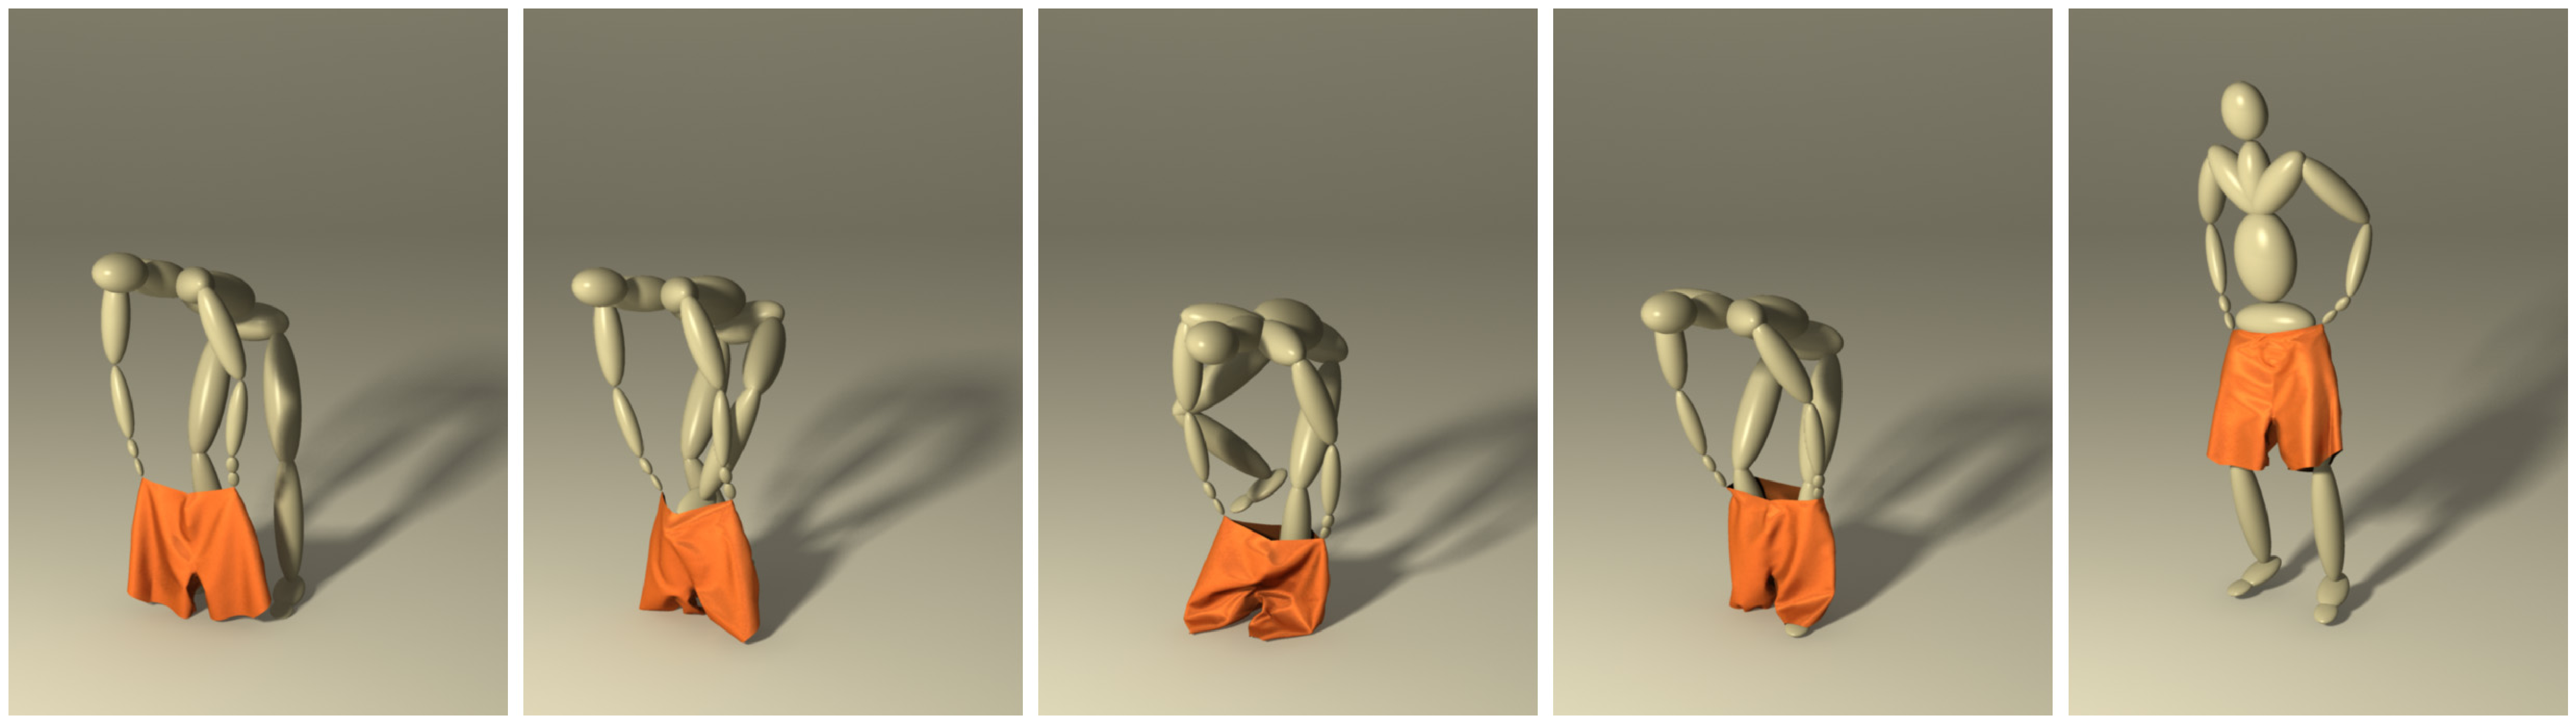
\includegraphics[width=\textwidth]{images/shortsStanding}
  \caption{A character puts on a pair of shorts in a standing pose.}
  \label{fig:shorts2}
\end{figure*}

\begin{figure*}[!t]
  \centering
  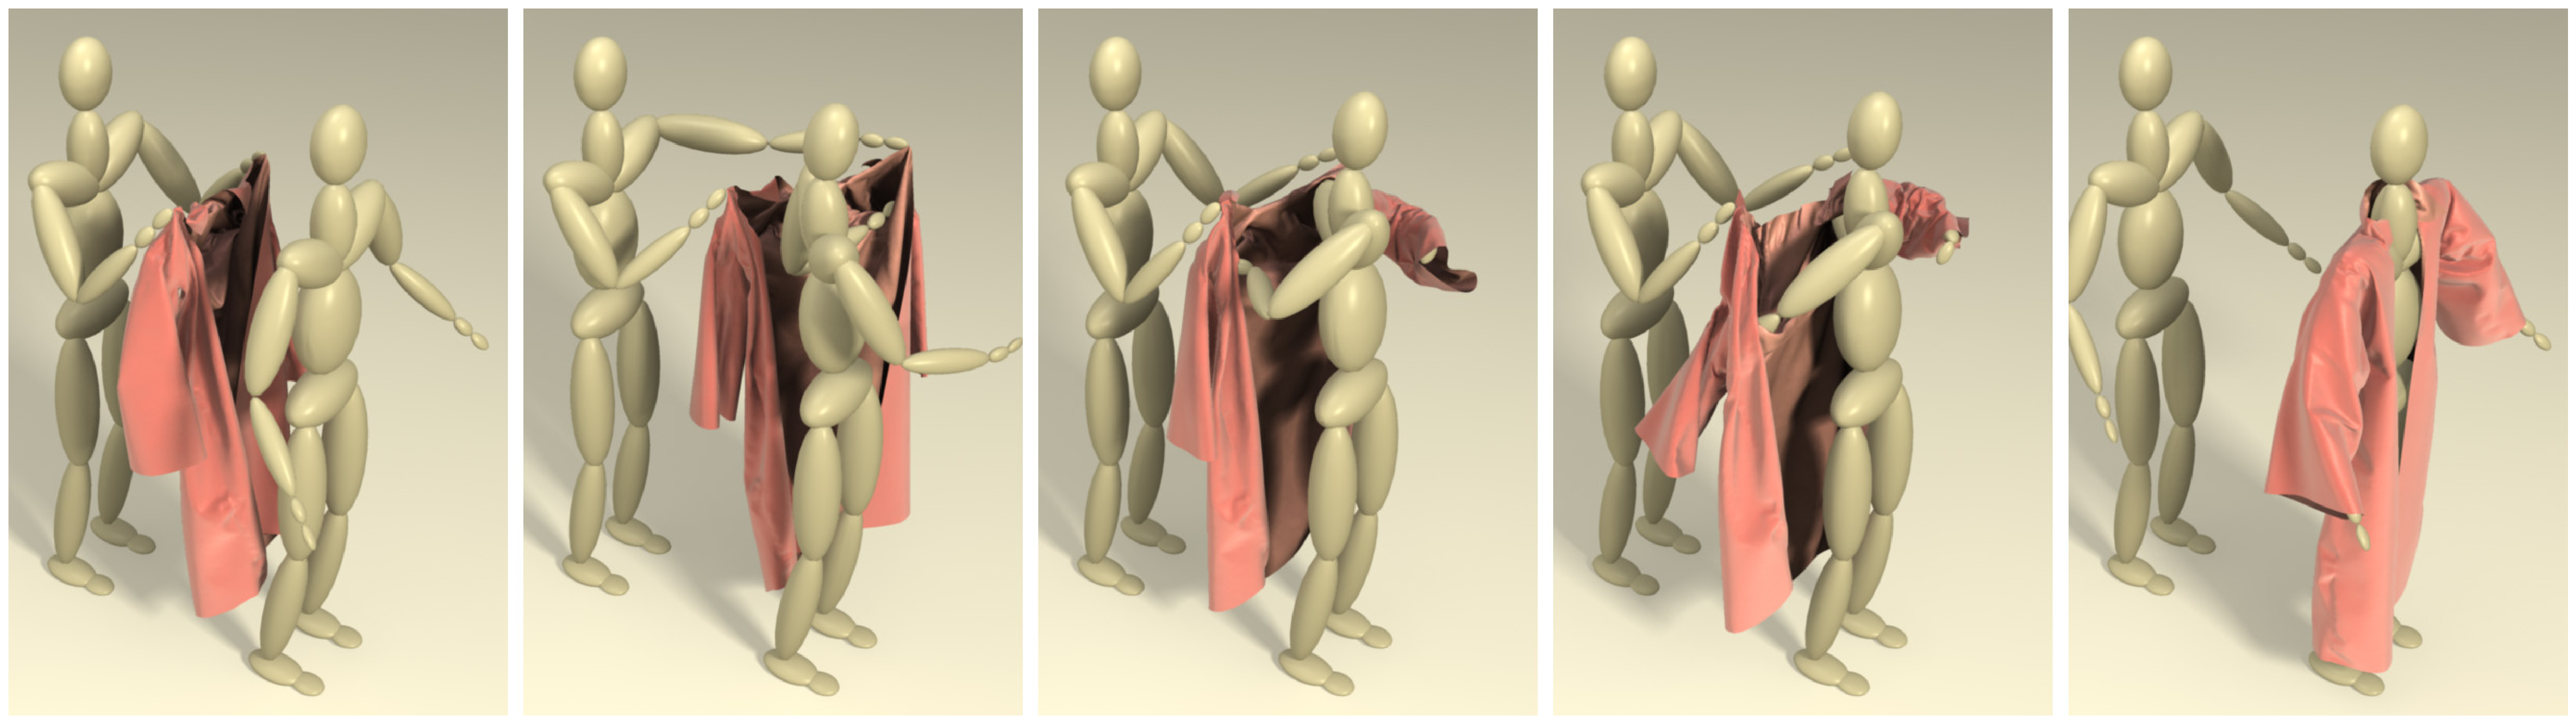
\includegraphics[width=\textwidth]{images/robe}
  \caption{A character puts on a robe with the help from another character.}
  \label{fig:robe}
\end{figure*}

\paragraph{Shorts.} Figure~\ref{fig:shorts1} demonstrates a character that
is putting on a pair of shorts in a sitting position. We used a motion
capture sequence as the reference motion in this example. The character
grips the waistband and leans forward by tracking the reference motion. He
first aligns his left foot with the waistband and then aligns it with the
bottom of the shorts' left leg. Similar alignment actions are applied to
the right foot. Once both feet are aligned with the desired features, the
character follows the reference motion to stand up and pull up the shorts.
The accompanying video shows that without the feedback control, the
character fails to put the feet into the shorts and ends up not wearing
the pants.

We also tested the generality of our system by using a different reference motion, in which we mocaped a person that is putting on a pair of shorts in a standing position. Despite the different style, we were able to reuse the action queue from the sitting shorts and successfully dress the lower body of the character (Figure \ref{fig:shorts2}).

\paragraph{Robe.} To show that our system can be used outside of the realm of self-dressing, we applied our method to an assisted dressing scene in which one character aids another in putting on a robe (Figure \ref{fig:robe}). The reference motion for this scene consists of five keyframes. First, the dressing character tracks the reference motion, twisting to the left and aligning his left hand with the armhole. After he straightens his arm into the sleeve, the assistant releases the cloth from his left hand. Dressing the second arm is similarly performed with both characters tracking to a pre-alignment position whereupon the dressing character aligns and straightens his arm and the assistant releases the sleeve. Note that in this example, the dressing control is only performed on the dressing character while the motion of the assistant is pre-scripted. It would be interesting future work to simulate and control both characters in an assisted dressing task.

% \input{discussion}
% \section{Conclusion}

We have presented a system that allows an animator to create motions
of people that are dressing.  By providing reference motion and an
action sequence, an animator has a fine degree of control over the
method and the style that a character uses to put on a garment.  We
have demonstrated the use of our method in creating a variety of
dressing animations, including putting on a jacket, a vest, pants
while sitting, pants while standing, and assistance in putting on a
robe.  They key technical aspects of our system are collision-free
inverse kinematics, path planning for limbs, and end effector path
planning using visibility feedback from the cloth. \karen{Probably
  want to revise the last sentence according to our recent discussion.}

There are several avenues for future work on animated dressing.  One
possibility is to incorporate dexterous manipulation of the cloth with our
current system.  Such an augmented system would allow a hand to properly
grip a sleeve, instead of ``gluing'' the hand to a portion of the cloth as
we currently do.  Another important aspect of dexterous manipulation that
we have not explored is the use of hands in fastening the garments, as is
needed to use buttons, zippers and laces.  As suggested in the Limitations
section, we might want a system that can figure out a high level dressing
strategy for a newly presented garment.  Such a system would likely need
to do some form of search across a variety of possible dressing
strategies.  There are potential improvements to cloth simulation that
could lead to higher quality dressing animation.  Current cloth simulators
do not handle multiple layers of cloth well, such as putting on a jacket
over a shirt.  The ability to handle tight contact between cloth and
the human figure would also increase the range of possible dressing
simulations.



\bibliographystyle{acmsiggraph}
\bibliography{template}

%\section{Appendix}

\jie{This should go to supplementary material.}
\begin{table}
	
  \begin{tabular}{|l|l|l|l|}
    \hline
    jacket 				& shorts 		& vest 			& robe \\
    \hline
    grip (right) 		& grip (right)	& grip (right)	& grip (left 2) \\
    track 				& grip (left)	& grip (left) 	& grip (right 2) \\
    align (left) 		& track 		& track 		& track\\
    Drag (left)			& align (left)	& release(left)	& align(left)\\
    release(right) 		& align (left)	& align (left)	& track\\
    track 				& track			& track			& release(left 2)\\
    align (right) 		& align (right) & grip (left)	& track\\
    Stretch	(right)		& align (right)	& release (right)& align (right)\\
    track 				& track 		& track			& track\\
    idle				& idle			& align(right)	& release\\
    					&				& release (right)& track \\
    					&				& Stretch (right)& \\
    					&				& track 		&  \\
    					&				& idle			& \\
    \hline
  \end{tabular}
  \caption{Action queue for various dressing scenes with only active actions.}
  \label{table:data}
\end{table}

\end{document}
